% With INS the position error grows cubically with time, due to the signal to noise ratio inherent to MEMS\ac{IMU}sensors \cite{Harle2013}. To compensate for this error, it is preferable that the\ac{IMU}sensor is mounted on the foot, as will be explained in \cref{sec:INS}. This placement requirement may limit usability. \\

%One advantage of the \ac{SHS}implementation is that the position error is proportional to the number of steps taken, but without the preference of using foot-based sensors, allowing for other sensor placements \cite{Diez2018b}.

% This section will outline the different PDR methods and focus on an \ac{SHS}approach to indoor localization.
\chapter{Related Work}
\label{chap:related work}
\textit{This chapter gives an overview of research related to inertial  sensor-based indoor localization. First, two different forms of such localization methods will be introduced. One will be deemed more appropriate for this thesis due to its applicability in a smartphone scenario and is analyzed further, where its different components will be outlined. Lastly, a method for orientation estimation is presented, which is an important component in localization. }


\section{Pedestrian Dead Reckoning}
\label{sec:relevant_research}
The person-focused indoor localization technique that uses \ac{MEMS} \ac{IMU} sensors is called inertial Pedestrian Dead Reckoning (PDR). Dead reckoning indicates that the output of the system will be the relative position change from a starting point \cite{Yu2018}. Within PDR there are two methods, namely \ac{INS} and \ac{SHS}. The INS mechanism integrates the \ac{IMU} signals directly \cite{Diez2018b}. \ac{SHS} is based on integrating the displacement vectors associated with each step taken during pedestrian locomotion \cite{Davidson2017}.  \par

\subsection{Inertial Navigation System}
\label{sec:rw-INS}
\begin{figure}[]
	\centering
	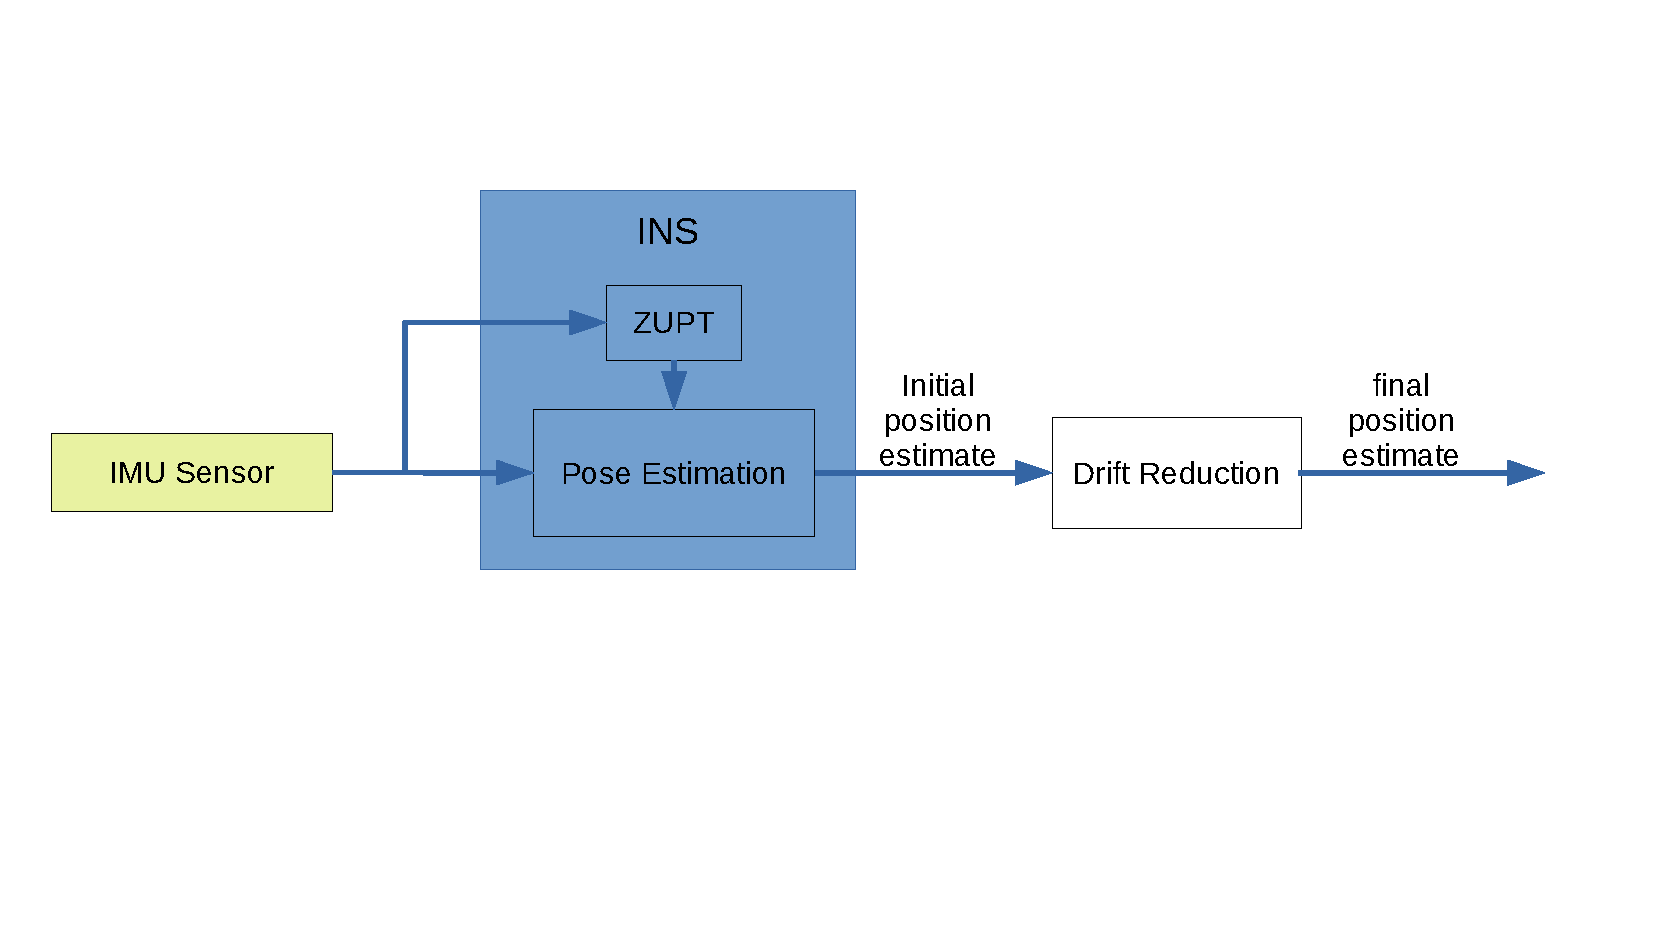
\includegraphics[trim=80 140 150 80, clip, width=0.8\linewidth]{images/INS_diagram}
	\caption{\ac{INS} pedestrian dead reckoning}
	\label{fig:ins_diagram}
\end{figure}
An Inertial Navigation System, as seen in \cref{fig:ins_diagram}, estimates pose, consisting of orientation and position, using sensor fusion algorithms. Examples of sensor fusion algorithms are the Extended Kalman Filter (EKF) and Complementary Filter (CF) \cite{Kok2017}. These methods are directly applied to the signals generated by  \ac{IMU} sensors \cite{Wu2019}, where position and orientation are found by integrating acceleration twice and integrating angular velocity once, respectively. This integration, in combination with the effects of noise and bias found in MEMS IMU, causes estimation errors to grow cubically with time for INS \cite{Harle2013}.  \par

A technique frequently used to compensate for the built-up error in INS is zero velocity update (ZUPT) and zero angular update (ZARU) \cite{Harle2013}. It utilizes the ability to detect time moments in which the sensor is stationary. Once detected, ZUPT uses the assumption that speed and angular velocity are zero at that time moment \cite{Wu2019,Harle2013}. This is a form of pseudo-measurement. Comparing the assumption with the model output of the sensor fusion algorithm, an error can be calculated and used to calibrate the sensor fusion estimate. This process is generally known as a measurement update and can occur every time a stationary period is detected.  Using this form of measurement update with INS, the error grows linearly instead of cubic with the number of steps \cite{foxlin2005pedestrian}.\par

Detecting brief stationary time periods during locomotion in pedestrian \ac{IMU} data is done easiest when the sensor is placed on the foot \cite{Diez2018,Davidson2017}. This is because a stationary period is much more pronounced in accelerometer data at this sensor location \cite{Yu2019,Wu2019}.  When walking, a foot periodically returns to an actual stationary state and stays there for a brief period of time, approximately 0.1 to 0.3 seconds \cite{Ren2016a}. This is the reason that most \ac{PDR} \ac{INS} research being foot-based \cite{Diez2018,Wu2019}. \citet{Solin2018a} overcome this preference for a foot-based system with a combination of several pseudo measurements, loop closure, and position fixes, opening up new possibilities for implementing INS as smartphone based localization method.

\subsection{Step and Heading System }

A \acf{SHS}, as shown in \cref{fig:shs_diagram}, is a form of pedestrian dead reckoning that detects steps, estimates step length, and the heading in which the step is taken. This position estimation can be represented by \cite{MunozDiaz2019}
\begin{equation}
	\label{eq:SHS_dynamic_model}
	\left(\begin{array}{l}
		p_{1,k+1} \\
		p_{2,k+1}
	\end{array}\right) 
	=
	\left(\begin{array}{l}
		p_{1,k} \\
		p_{2,k}
	\end{array}\right) 
	+l_{k} \left(\begin{array}{l}
		\cos \left(\phi_{k}\right) \\
		\sin \left(\phi_{k}\right)
	\end{array}\right),
\end{equation}

where $p_{1,k}$  and  $p_{2,k}$ represent the position in the $x$-axis and $y$-axis at time step  $k$, respectively. Furthermore $l_{k}$ stands for the step length, while $\phi_{k}$ is the step heading of the pedestrian at time step $k$.
Similarly to INS with ZUPT measurement updates, \ac{SHS} position error is proportional to the number of steps taken. The largest difference is that this error growth does not require detecting stationary moments and therefore does not have a preference for using foot-based sensors, as is the case with INS and ZUPT. This allows for other sensor placements \cite{Diez2018b}. However, other of sources of error can be introduced due to errors in the detection of steps and their length estimation. \par 
Since other sensor placements are possible, \ac{SHS} is the PDR technique often used with smartphones as the base for sensing \cite{Kang2015}. This therefore seems to be the more appropriate method to implement, and will be the \ac{PDR} method that will be focused on in the rest of this thesis. The components of \ac{SHS} will be treated in further detail in \cref{sec:shs_components}.

\label{sec:rw-SHS}
\begin{figure}[H]
	\centering
	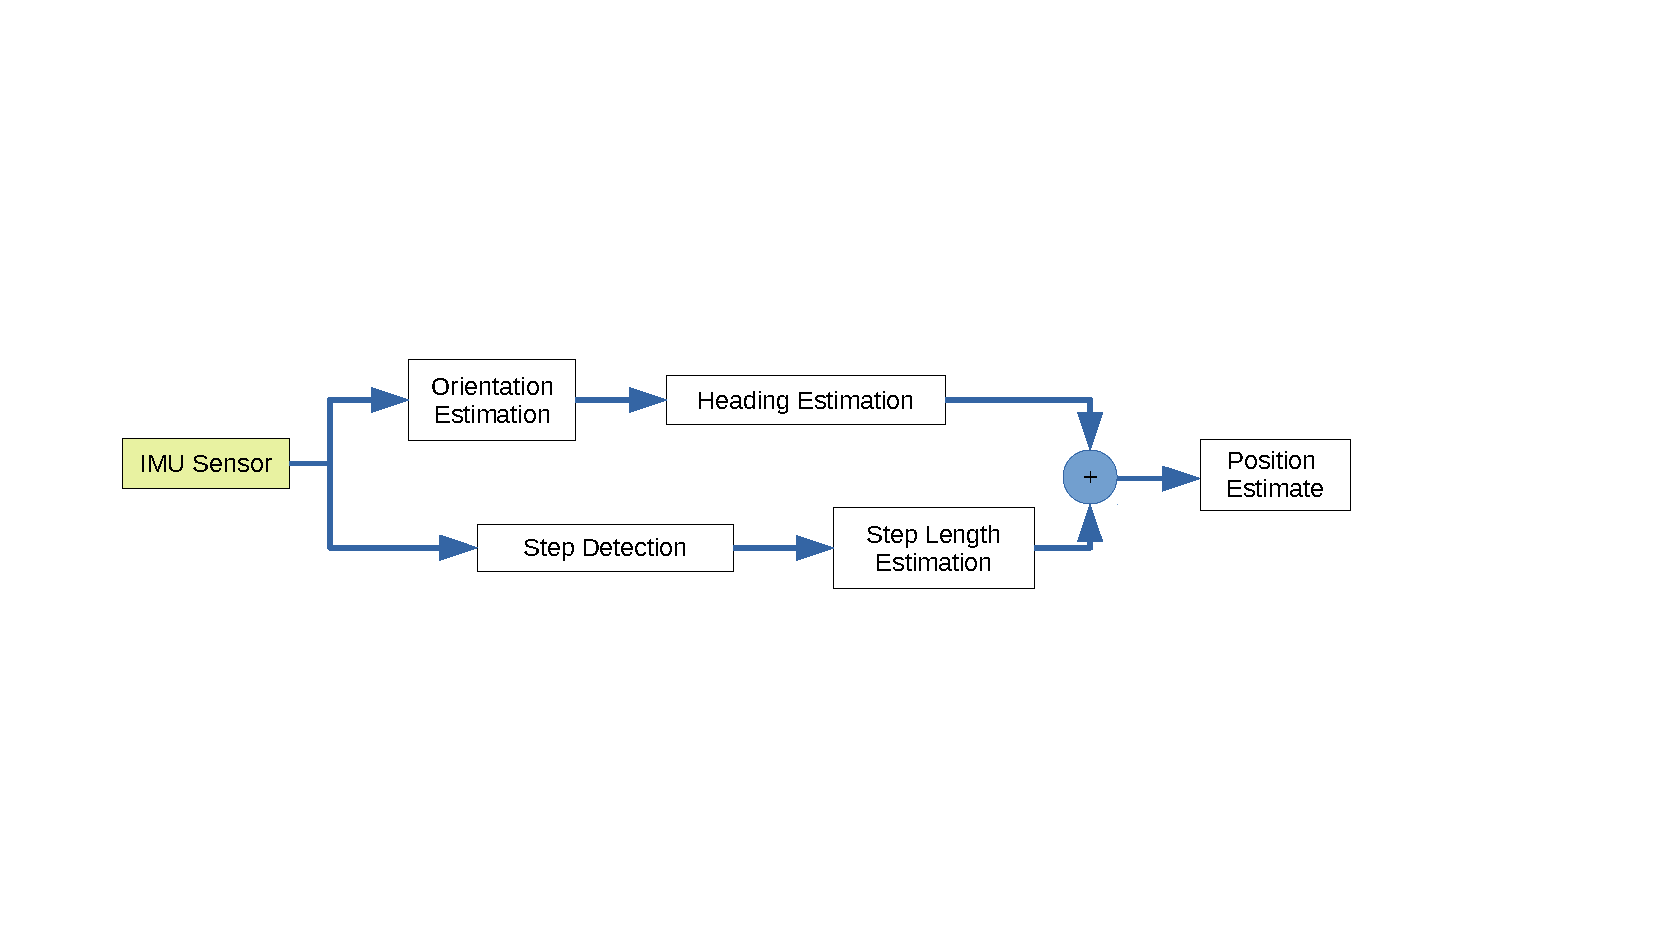
\includegraphics[trim=40 120 140 100, clip,width=\linewidth]{images/shs_diagram}
	\caption{\ac{SHS} pedestrian dead reckoning}
	\label{fig:shs_diagram}
\end{figure}

%This indicates that this technique is appropriate for further investigation in answering the thesis research questions.\\

%This method can be combined with a Particle Filter \cite{Koivisto2016, Jackermeier2018}. This allows for more constraints, consequently requiring less particles for localization.
\section{Drift Reduction through Spatial Context}
\label{sec:rw-drift_reduction}
PDR methods alone accumulate error with time and are therefore not ideal for long-term pedestrian tracking \cite{Hardegger2012}. Drift reduction methods can be used to try and compensate for this error \cite{MunozDiaz2019a}.  These methods use additional information to improve the estimate. One approach is by complementing the \ac{PDR} solution with infrastructure dependent techniques that use external signal generation to acquire additional position information \cite{Qian2015}. An infrastructure independent source of information is spatial context, where the geometric and topological characteristics of the indoor environment are exploited \cite{Gu2019}. Spatial context can be used to restrict the position estimate, through assumptions or simplifications. Spatial context methods often use spatial models, maps, and landmarks, which will be handled individually next, followed by the Particle Filter, a technique able of combining all three forms spatial context. \par

\subsection{Spatial Models}

Spatial models simplify the indoor environment through graph or grid models. For graph models the indoor environment is represented by a set of links and nodes, along which the position estimate is restricted \cite{Davidson2017,Jackermeier2018}. Grid models split the whole map into a grid where each cell represents the probability of a tracked target being within it \cite{Gu2019} and where the estimate can move between cells.\par 

\subsection{Maps}

A map describes the indoor layout of building, often in the form of a floor plan \cite{Gu2019}. Examples of using maps as drift reduction include restricting the movement to be parallel to the outer walls of a building \cite{Abdulrahim2011}, where the assumption was made that hallways and rooms will be parallel to these walls. Trajectories can also be matched to  the indoor environment, respecting the different spatial constraints \cite{Gu2019}. Another option is to propagate the estimate within a representation of the indoor environment \cite{Qian2015}. The estimate will then have to adhere to the physical inability of crossing certain structures such as walls and furniture.\par

\subsection{Landmarks}

Landmarks are specific locations with a unique footprint detectable in sensor data. When the user visits a landmark and this is detected, the location of the landmark can be used to calibrate the position estimate of the user, hence compensating drift \cite{Diaz2017}. Depending on the sensors available, different landmarks become detectable. Examples of landmarks are doors and stairs \cite{Diaz2017,Gu2019,Torok2014}, but also unique magnetic footprints \cite{MunozDiaz2019}, and electromagnetic signal footprints \cite{Gu2019}. Activity recognition on sensor data can also be used to detect interaction with location dependent landmarks within the environment \cite{Hardegger2012, Hardegger2016}.  Some landmarks can be easily determined beforehand, through the use of available building blueprints \cite{Gu2019}. 

\subsection{Particle Filter}
\label{sec:rw-pf}

The Particle Filter is a sensor fusion method able of encapsulating all the above spatial drift reduction methods. Sensor fusion entails using multiple sources of information to determine state estimates of modeled systems. The general filter approach will be explained and its relevance to indoor localization through spatial context will follow.\par
An overview of the generic Particle Filter can be found in \cref{algo:rw-bootstrap_PF}.  The filter uses a finite amount of particles $N$, representing state realizations $x^i$ where $i = 1,...,N$. These particles have an associated weight $\omega^i$ and, combined with their states, generate a posterior probability distribution. \par 
Three recursive steps are completed within the filter, including measurement update, resampling, and time update \cite{Wu2019,Woodman2008}, which will be treated next.

\subsubsection{Measurement Update}
During a measurement update, each particle's weight is changed according to how its state evaluates against constraints or system evaluation functions. The likelier the particle is within the system constraints, the higher the particle's weight become. This is represented by

\begin{equation}
	\omega^i_{k|k} = \frac{1}{c_k} \omega^i_{k|k-1} p(y_k|x^i_k),
\end{equation}\\
where the normalization weight is given by
\begin{equation}
	c_{k}=\sum_{i=1}^{N} w_{k | k-1}^{i} p\left(y_{k} | x_{k}^{i}\right).
	\label{eq:PF_probability density}
\end{equation}

where $p(y_k|x_k^i)$ is the conditional probability of a measurement $y$ given the state of particle $i$, at time step $k$.

\subsubsection{Resampling}
Resampling is used to select a new group of particles based on the weights of the current particles. The higher the weight of a particle is, the more likely it will be resampled. A particle can even be resampled multiple times. \par 
There are multiple methods that can be used for resampling including multinomial, stratified, systematic, and	residual resampling \cite{hol2006resampling,gustafsson2010statistical}. \citet{hol2006resampling} conclude that  systematic resampling is the best considering resampling quality and computational complexity. Systematic resampling is defined as 

\begin{align}
	x^{i*} &= x(F^{-1}(u^i)), \\
	u^i &= \frac{(i-1) + \tilde{u}}{N}, \qquad \tilde{u} \sim \mathcal{U}[0,1).
\end{align}	

Here $x^{i*}$ represents the newly sample particle with index $i$, and $F^{-1}$ represents the generalized inverse of the cumulative probability distribution of the normalized particle weights. It returns the index of a particle in the particle list, the state of which is returned by $x(*)$. Once the particles are resampled the particle weights are set to $\omega^i_{k+1|k} = 1/N$ . \par
Resampling inevitably destroys information and therefore increases uncertainty by the random sampling \cite{gustafsson2010particle}. Resampling should therefore occur only when it is needed. \citet{gustafsson2010statistical} proposes the use of  \textit{effective number of samples} to trigger a  resampling. This can be calculated as 
\begin{subequations}
	\begin{equation}
		N_{\mathrm{eff}}=\frac{1}{\sum_{i=1}^{N}\left(w^{i}\right)^{2}},
	\end{equation}
	
	where
	
	\begin{equation}
		1 \leq N_{\mathrm{eff}} \leq N.
	\end{equation}
\end{subequations}

The resampling condition can then be defined as $N_{\mathrm{eff}} < N_{th}$, where the threshold $ N_{th} $ can be placed at $2N/3$ \cite{gustafsson2010statistical}, with $N$ being the total number of particles. \par 

\subsubsection{Time Update}
Every time step within the Particle Filter, all particles are propagated according to a proposal distribution \cite{gustafsson2010particle}. Within the standard version of the filter, the conditional prior of the state vector is used. 

\begin{equation}
	x_{k+1}^{i} \sim p(x_{k+1}|x^i_{k}).
\end{equation}


\begin{algorithm}[H]
	\SetAlgoLined
	\caption{Bootstrap Particle Filter}
	\label{algo:rw-bootstrap_PF}
	Choose the number of particles N.\\
	\underline{initialization:}
	Generate 
	\begin{subequations}
		\begin{equation}
			x^i_1 \sim p_{x1}, \qquad i = 1,...,N
		\end{equation}
		and let
		\begin{equation}
		 \omega^i_{1|0} = 1/N
		\end{equation}
	\end{subequations}
	\;
	\For{k = 1,2,...}{
		\underline{Measurement update:}\\
		\begin{subequations}				
				\begin{align}
					\omega^i_{k|k} &= \frac{1}{c_k} \omega^i_{k|k-1} p(y_k|x^i_k),\\
					c_{k} &= \sum_{i=1}^{N} w_{k | k-1}^{i} p\left(y_{k} | x_{k}^{i}\right)
					\label{eq:PF_probability density}
				\end{align}			
		\end{subequations}
			\underline{Resampling:}\\
			take $N$ samples with replacement from the set $\{x^i_{1:k}\}^N_{i=1}$ where the probability to take sample $ i $ is $\omega^i_{k|k} = 1/N$.\\
			\underline{Time update:}\\
			Generate predictions according to the dynamic model, using realizations of the process and measurement noise.
			\begin{equation}
				\label{eq:PF_dynamic model}
				x_{k+1}^{i} \sim p\left(x_{k+1}^{i} | x_{k}^{i}\right)
			\end{equation}
		
	}
\end{algorithm}


\subsubsection{State Estimation}

The posterior distribution is the primary output of a Particle Filter \cite{gustafsson2010particle}. For state inference purposes a single point estimate is more convenient \cite{Saha2009}. The weights and positions of the particle cloud can be used to generate a single point estimate \cite{gustafsson2010particle}. There are different ways of defining the eventual position estimate. The maximum a posteriori (MAP) estimate picks the particle with the highest weight from the posterior distribution \cite{Saha2009}, while the  minimum mean square error (MMSE) estimate calculates a weighted mean \cite{gustafsson2010particle,Saha2009}.\par 

\subsubsection{Spatial Context Particle Filter}
For indoor localization, the particle filter can use spatial context as either a form of measurement update or time update. Particles will move through a representation of the indoor environment, defined by a spatial model \cite{kihlberg2012map, Qian2015}. They will adhere to a motion model defined by the output of the eventual \ac{SHS}, consisting of step length and direction.\par 

With spatial context, a measurement update for indoor localization can take different forms \cite{Gu2019}. With map information, the measurements updates can evaluate the position of each particle with the indoor constraints \cite{Qian2015}. Particles that violate these constraints will be disregarded, limiting state estimation to within the defined constraints. Detecting landmarks allows for the landmark positions to be compared with particle positions, with closer particles receiving higher weights \cite{Shang2015}.  \par 

The Particle Filter is able to estimate non-linear posterior densities, allowing for multimodal distributions \cite{gustafsson2010particle,kihlberg2012map}. Multimodal distribution refers to distributions with multiple maxima in the probability density function. This allows the Particle Filter to have multiple hypotheses for the system that it is modeling. In the case of indoor localization, this translates to indicating that there are two position estimates that are equally likely based on the information that the filter has received so far. This can occur due to symmetry in the indoor environment  \cite{Woodman2008}.


\newpage
\section{Step and Heading System Components}
\label{sec:shs_components}

\cref{sec:rw-SHS} concluded that the \acl{SHS} approach was to be the \ac{PDR} method to focus on further for a smartphone based system. Within the \ac{SHS} method there are three components to consider: step detection, step length estimation and step heading estimation. The following section will treat each component of this system individually, outlining the different possibilities for it to fulfill its role. \par 

\subsection{Walk and Step Detection}
\label{sec:rw - step detection}
Walk detection is determining from \ac{IMU} sensor data if a walking activity is being performed, whereas step detection is deciding when a step is taken during this activity. \\
Techniques such as feature classification, frequency domain analysis, and time-domain thresholding can be used to detect the two activities \cite{Yang2014}. An overview of techniques  is summarized in \cref{tab:step_detection_comparison}. Naturally, each form of walk and step detection has its advantages and disadvantages.\par

\subsubsection{Time-domain analysis}
 Time domain analysis often uses the acceleration norm, making it robust to sensor orientation \cite{Davidson2017}. Its simplest form, thresholding, is simple to implement. The problem with thresholding is that it is difficult to determine the optimal threshold value, as it can vary between users, surfaces, and even shoes \cite{Brajdic2013}.  

\subsubsection{Frequency domain analysis} 
Frequency domain analysis is often  also invariant to sensor placement \cite{Brajdic2013} since the periodicity in the norm of acceleration during pedestrian locomotion stays the same for different carrying modes. This therefore also makes frequency analysis robust to sensor orientation. Frequency methods have the disadvantage that they are only able to detect periodic motion \cite{Davidson2017}. \par 

For both frequency and time domain-based analysis, it is possible that certain motions, aside from the desired motion, can cross the threshold and generate false positives. In addition, frequency analysis and template matching, a more advanced time based method, will have a certain computational overhead to consider \cite{Davidson2017, Harle2013}. 

\subsubsection{Feature classification methods} 
Feature classification methods use characteristics in accelerometer traces to classify steps, using forms of machine learning \cite{Brajdic2013}. These methods have the advantage that they can determine relations from labeled data automatically, removing a need for humans to define them. This is also a disadvantage as it requires labeled data, the gathering of which can be a labor-intensive process \cite{Bulling2014}. Furthermore, the models they determine will depend on the data gathered. This may lead to over-fitting \cite{Bulling2014}. In addition, certain classification methods may require significant processing power, limiting the platforms on which it can perform \cite{Yang2014}.

	\begin{table}[]
	\centering
	\small
	\renewcommand{\arraystretch}{2}
	\begin{tabularx}{\linewidth}{ P{20mm}| P{17mm} L}
		\toprule
		\thead[lb]{Form} & \thead[lb]{Technique}	&   \thead[c]{Explanation}	\\
		\midrule			
		\multirow{4}{17mm}{Time domain analysis}& Threshold & Acceleration magnitude is monitored for the passing of certain values or sign changes, in the case of Zero Crossing method \cite{Davidson2017,Harle2013}. Typically determines when the foot is on the floor \cite{Harle2013}, but has also been applied to pitch angle of the upper leg, where the sensor has been placed \cite{Diaz2014a}. In some instances, the thresholds are altered adaptively, for example through different motion mode detection or information gathered from the previous step \cite{Wu2019}.\\ \cline{2-3}
		&(Windowed) Peak Detection & Recognizes local maximum or minimum on acceleration magnitude caused by foot impact on the floor, often within a sliding window \cite{Susi2013}. Generally combined with thresholding, which is one of the simplest combination used with \ac{SHS} \cite{Davidson2017}. \\ \cline{2-3}
		& Auto-correlation (Template Matching) &  Finds correlation of a signal with a time-shifted copy of itself. It leverages the strong cyclic nature of bipedal locomotion \cite{Harle2013}. Since the lag for the highest correlation is not known beforehand, an interval is often swept and correlation values compared. \\ \cline{2-3}
		&Dynamic Time Warping & Similar to autocorrelation, it measures the similarity between two waveforms from accelerometer data \cite{Davidson2017}, These waveforms can both come from the data or one could be a stride template generated offline. A non linear mapping between the two methods is made, resulting in a DTW distance. A smaller distance indicates higher similarity \cite{Davidson2017}.  \\ \hline
		\multirow{2}{17mm}{Frequency domain analysis} & Short Term Fourier Transform & Transforms acceleration signal of successive windows of data into the frequency domain. For spectral analysis, a subset containing a stride (two steps) is required to determine the frequency \cite{Harle2013}.  \\ \cline{2-3}
		&Wavelet Decomposition & Acceleration magnitude is split into low and high-frequency components, from which the dominant frequency is assumed to be the walking frequency. Iterating this process on the resulting low-frequency signal approximation, a smoother shaped dominant low-frequency signal is generated. The frequency of this signal corresponds to walking cadence \cite{Davidson2017}. \\ \hline	
		\multirow{2}{17mm}{Feature classification} & Hidden Markov Model & Uses gait cycles segmented into different states of a state machine, to determine if a step has been taken \cite{Ren2016a}. Thresholds can be used to induce a state change. If a full state machine cycle is achieved, a step is detected.\\ \cline{2-3}
		& K Nearest Neighbors & Uses labeled data containing features from successive time windows and compares a new time window with its features. It finds the labeled data whose features are most similar. This new set then receives its label. \\
		\bottomrule
	\end{tabularx}
	\caption{Overview of different step detection methods using inertial sensors.}
	\label{tab:step_detection_comparison}
\end{table}

\citet{Brajdic2013} tested and compared a variety of algorithms for both walk detection and step detection on unconstrained smartphones. The article reviews techniques with different levels of complexity from a variety of different papers. In order to compare the different techniques, the researchers collected a large dataset from 27 test subjects. Each subject held the smartphone in six different carrying modes: in hand in front of user (idle and with device interaction), in a front pocket, in a back pocket and in a handbag or backpack. A ground truth was generated by video recording each session and manually counting the amount of steps taken. Using this dataset a comparison is made between the nine techniques in \cref{tab:step_detection_comparison}.\par 
The paper concludes that for the generated dataset, the best step counting results were obtained using the Windowed Peak Detection, Hidden Markov Model, and Wavelet Decomposition. Each had a median error of about 1.3\%.\par 
Considering the relative simplicity of the technique, the authors recommended Windowed Peak Detection as the most efficient algorithm for step detection. The best walk detection algorithms were short-term Fourier transform, normalized autocorrelation, and thresholds on either standard deviation or signal energy. Again for their simplicity, the threshold approaches were recommended. \par
\citet{Salvi2018} build upon the conclusions and recommendations of \citet{Brajdic2013}, with the aim of further optimizing the Windowed Peak Detection algorithm and its parameters. The algorithm is based on the approach of \citet{Palshikar2009} and consists of 5 stages run in series. These are pre-processing, filtering, scoring, detection and post processing. An exhaustive grid search across the parameter space was performed to find the optimal set for step detection. Using these parameters, an average accuracy of $95\% \pm 4.5\%$ in counting the correct number of steps taken was reached, considering all the carrying modes.

%These results make this approach 


\subsection{Step Length Estimation}
\label{sec:step_length_estimation}
From subsequent step detections, step length can be estimated, generating a displacement vector. \citet{Collins2013a} found that increasing step speed leads to larger step lengths, while step speed can have slow and spontaneous fluctuations depending on the motion mode. In addition, step size depends on the physical characteristics of the user and on their walk strategy, which can be different per individual \cite{Diez2018}. These discrepancies indicate that using a simple average step length for every pedestrian could result in quick accumulation of error. \citet{Diez2018} categorizes step length estimation methods into integration based and model-based methods. \par

Theoretically, the double integration of the \ac{IMU} acceleration signal is the best approach to step size estimation, using the INS approaches outlined in chapter \secref{sec:rw-INS}. This would give a direct measurement of displacement. It does not require any modeling, assumptions, or person-specific calibration \cite{Diez2018}. However, since it would be an INS approach, it suffers from the same drift problems, as expressed in \cref{sec:rw-INS}, and would require the same solutions. This approach therefore benefits from having the sensor located on the foot. \par 

Analytical models can be made of human mobility based on geometrical relationships of body composition, angles, and displacement of body parts. Such methods use regression to determine relationships to step length.  One of the largest disadvantages of a model-based approach is that human proportions are not uniform, requiring approximations and/or some form of calibration for the model to be accurate \cite{Diez2018}. Model based approaches are often either frequency, acceleration or angle based, sometimes even a combination of multiple approaches \cite{Vezocnik2019}. Often there are tunable parameters within the different models that need to be calibrated.

\citet{Vezocnik2019} compared different existing step length estimation algorithms using inertial sensors. The review focuses on the model based methods applicable to smartphone use. This means methods that do not require training and do not require the sensor to be placed on the foot. This, therefore, excludes machine learning and INS systems. The robustness of the methods was tested by having the smartphone carried by multiple people and in different carrying modes. This includes the smartphone in a front pocket, in a bag, in the hand with the phone screen parallel to the floor, and in hand will swinging the carrying arm. \par 

A differentiation was made between global variables and personal ones, where the former applies the same set of variables to all users, while the latter are tuned per person. For global parameters, the method of \citet{Tian2016} proved to be the best, defined as

\begin{equation}
	\label{eq:Tian2016_sle}
	\text{step size} = K_1 h \sqrt{F}.
\end{equation}

Here $K_1$ is a tunable parameter, $h$ is the height of the user and $F$ is the step frequency. This method reported an average error of  4.59 \% for personalized variables and 6.96 \% for global ones. \par 

For personally tuned variables, the method of \citet{Weinberg2002} was best. This is an inverted pendulum model in which the human center of mass is used, located approximately at the pelvis. The center of mass rotates as an inverted pendulum when taking a step. This is followed by a forward horizontal displacement when both feet are on the ground \cite{Diez2018}. The model is given by

\begin{equation}
\text{step size} =K_2 \sqrt[4]{A_{\max }-A_{\min }}.
\label{eq:weinberg_stepsize}
\end{equation}

Here $A_{\max}$ is the largest measured acceleration measured within a step interval, while $A_{\min}$ is the smallest. $K_2$ is a calibration variable  \cite{Weinberg2002,Diez2018}. The model had an average error of  10.64 \% for global variables and  3.60 \% for personalized \cite{Vezocnik2019}.

\subsection{Step Heading Estimation}
\label{sec:rw-step_heading_estimation}
Step heading determines the direction in which a detected step is taken. This is not necessarily the orientation of the smartphone, since the device can be carried in different carrying modes and therefore different orientations. For step heading, and orientation estimation in general, different coordinate frames are important to consider in such cases. First the relevant coordinate frames and their notation are introduced, after which they will be used to explain different heading estimation techniques. \par 

\subsubsection{Coordinate Frames}
There are two coordinate frames that are of importance for localization: the body frame and the navigation frame. The body frame ($\mathrm{b}$) is the coordinate frame of the IMU, the origin of which is at the center of the triaxial accelerometers found in the device \cite{Kok2017}. The navigation frame ($\mathrm{n}$) is the geographical frame in which the user is moving. It is also the frame in which the pose of the body frame, consisting of orientation and position, is to be determined. For a localization application the navigation frame is considered stationary \cite{Kok2017}.\par

In notation, a superscript on a vector is used to indicate in which coordinate frame it is expressed. For example, $x^\mathrm{n}$ is the vector $x$ expressed in the navigation frame. A double superscript indicates an orientation mapping from one frame to another. For example, $R^\mathrm{nb}$ is a rotation matrix that maps from the body frame to the navigation frame.

\subsubsection{Heading Estimation Methods}
Step heading estimation requires knowing the orientation of the sensor with respect to the navigation frame and from there determining in what direction the sensor is moving. It is currently the component within \ac{SHS} whose performance is the most limiting for positioning purposes \cite{Diez2018b, Qian2013,Combettes2017}. IMU orientation estimation is done through sensor fusion, a process in which data from multiple sensors are combined for state estimation. An often used method will be outlined in detail in \cref{sec:rw-orientation_estimation}.
Once the sensor orientation is estimated there are two approaches to determining heading, one that unconstrained smartphone positions and the other for constrained positions. 

For unconstrained phone position three techniques are often used: Principal Component Analysis (PCA), Forward and Lateral Accelerations modeling (FLAM), Frequency analysis of Inertial Signals (FIS). A brief overview of each method will be given. For more detailed information on these techniques, the reader is refered to \cite{Combettes2017}.

PCA is the technique often used for unconstrained smartphones. It assumes that the variance over a gait cycle of the horizontal acceleration is maximum along the heading direction \cite{Combettes2017}. It attempts to maximize a horizontal axis across acceleration measurements . FLAM uses a predefined acceleration template defined from a known orientation in the navigation frame with respect to the movement of the user. Finding the heading then consists of maximizing the correlation of the generated template with the estimated acceleration data from the IMU \cite{Combettes2017}. FIS is a technique that tries to determine the direction that maximizes the spectral density of accelerometer and gyroscope signal energy at step and stance frequency. 

\citet{Combettes2015} have done a comparison on the different unconstrained heading estimation method introduced. From their results they have deemed all three not accurate enough for being used alone in an intertial \ac{PDR} setting for heading estimation. They determined that performance of the different technique varies largely depending on the orientation of the unconstrained device, sometimes having errors up to 28 degrees. This reasoning is likely why the unconstrained solutions are often combined with the constrained ones.

For the constrained method, the phone is limited to one or more carrying modes or poses. The easiest approach is constraining the device to one carrying mode typical of smartphone use, such as in front, in hand, with the screen point up from the ground \cite{Deng2016}. Here the assumption can be made that a change in phone orientation also represents a change in heading direction. Extending this to more carrying modes can be achieved by determining the carrying mode of the smartphone through machine learning algorithms \cite{Lee2019, Sun2015a}. Depending on the detected carrying mode a different heading estimation method can be used. In positions such as holding it in front of the body or calling, a constant offset can be calculate and subtracted to determine the heading \cite{Sun2015a}. For other positions such as in the front pocket or while held in a swinging arm some form of Principle Component Analysis \cite{Deng2016,Lee2019,Sun2015} is performed.\par



\section{Inertial based Orientation Estimation}
\label{sec:rw-orientation_estimation}
As stated in the previous section, heading estimation within a \acl{SHS} requires knowing the orientation of the \ac{IMU} sensor with respect to the navigation frame. Orientation estimation through \ac{IMU} sensors has been available for some time, being experimentally invented for stabilization and navigation of aircraft and missiles \cite{titterton2004strapdown}. In these high performance settings, sensor fusion techniques are applied to take any eventual sensor noise from the instrumentation into account to produce accurate estimates. This has allowed for inertial-based tracking over long periods of time \cite{Harle2013}. Regrettably, the sensor constructions for these settings are too large and costly for widespread use.\par  

It is the introduction of \ac{MEMS} \ac{IMU} sensors, measuring the same phenomenon but with a small form factor and cheap cost, that has made the same orientation sensor fusion techniques applicable to new situations, such as indoor localization.  The largest difference between the experimental use case and this new one is the larger susceptibility of MEMS to sources of error and more significant imperfections in the sensors, leading to a difference in sensitivity along different axis. \par 

The following section explains the Extended Kalman Filter approach, a sensor fusion technique often used with PDR \cite{Michel2015a,Michel2018, Diaz2014}. It first treat relevant orientation parametrizations and motion models needed for in the filter. This is followed by sensor calibration. At the end of the section, the EKF process is outlined within the orientation estimation framework.


\subsection{Orientation Parametrization}
While position is often represented by a point in a 3D orthogonal axis frame, orientation has different parametrizations, each able to map to one another, an overview of which can be found in \cref{chap:appen-orientparam}. The Extended Kalman Filter in this section uses rotation matrices ($R$) and quaternions ($q$) to calculate orientation from inertial sensors.

\subsubsection{Rotation Matrix}
Rotation matrices $R \in \mathbb{R}^{3 \times 3}$ have the following properties:

\begin{equation}
	\label{eq:rot_mat_properties}
	R R^{\top}=R^{\top} R=I_{3}, \quad \text { det } R=1.
\end{equation}

These matrices can be used to express a vector $x \in \mathbb{R}^{3}$ in frame $v$ to frame $u$ as 

\begin{equation}
	\label{eq:rot_mat_rot_x}
	x^{\mathfrak{u}}=R^{\mathfrak{u} \mathrm{v}} x^{\mathrm{v}}.
\end{equation}

Transposing a rotation matrix represent a rotation back to it's experimental coordinate frame:
\begin{subequations}
	\begin{align}
		\label{eq:rot_mat_trans}
		x^{\mathrm{v}}&=\left(R^{\mathrm{uv}}\right)^{\top} x^{\mathrm{u}},\\
		&=R^{\mathrm{vu}} x^{\mathrm{u}}.
	\end{align}
\end{subequations}

\subsubsection{Unit Quaternion}
A unit quaternion is an orientation parametrization frequently used by attitude estimation algorithms. This is because it is free of non-singularity in attitude representation \cite{Hashim2019}, also known as wrapping. A unit quaternion can be described by

\begin{equation}
	\label{eq:unit_quarternion}
	q=\left(\begin{array}{llll}{q_{0}} & {q_{1}} & {q_{2}} & {q_{3}}\end{array}\right)^{\top}
	=\left(\begin{array}{l}{q_{0}} \\ {q_{v}}\end{array}\right), 
	\quad q \in \mathbb{R}^{4}, 
	\quad\|q\|_{2}=1.
\end{equation}

A rotation of vector $x$ using quaternions between two frames, from $v$ to $u$, is indicated as

\begin{equation}
	\label{eq:quat_rot}
	\bar{x}^{\mathrm{u}}=q^{\mathrm{uv}} \odot \bar{x}^{\mathrm{v}} \odot q^{\mathrm{vu}},
\end{equation}

where $q^{\mathrm{vu}} = \left(q^{\mathrm{uv}}\right)^{\mathrm{c}}$, with the latter representing the quaternion conjugate, defined by 

\begin{equation}
	\label{eq:quat_conjugate}
	q^{\mathrm{c}}=\left(\begin{array}{c}{q_{0}} \\ {-q_{v}}\end{array}\right).
\end{equation}

$\bar{x}^u$ represents the quaternion version of the vector $x^u \in \mathbb{R}^3$, as

\begin{equation}
	\label{eq:quat_vec_ref}
	\bar{x}^u=\left(\begin{array}{l}{0} \\ {x^u}\end{array}\right).
\end{equation}


The $\odot$ operator describes quaternion multiplication, defined by

\begin{equation}
	\label{eq:quat_multiplication}
	p \odot q=\left(\begin{array}{c}{p_{0} q_{0}-p_{v} \cdot q_{v}} \\ {p_{0} q_{v}+q_{0} p_{v}+p_{v} \times q_{v}}\end{array}\right).
\end{equation}

Since both parametrizations represent an orientation, they can be mapped from one to another and vice versa. More information on these mappings can be found in \cref{chap:appen-orientparam}.

\subsection{Motion and Measurement Models}
\label{sec:motion_and_measurement_models}
The signals generated by an \ac{IMU} can be combined such that orientation can be deduced. For many sensor fusion algorithms this is generally done by defining motion and measurement models, which when combined form a state space representation. Using the \ac{IMU} signals, the orientation state space can be defined \cite{Kok2017} as 
\begin{subequations}
	\begin{align}
		\label{eq:orient_dynamics}
		q_{k+1}^{\mathrm{nb}} &=q_{k}^{\mathrm{nb}} \odot \exp _{\mathrm{q}}\left(\frac{T}{2}\left(y_{\omega, k}+e_{\omega, k}\right)\right), 	\\ 
		\label{eq:orient_acc_measure}
		y_{\mathrm{a}, t} &=-R_{k}^{\mathrm{bn}} g^{\mathrm{n}}+e_{\mathrm{a}, k},\\ 
		\label{eq:orient_mag_measure}
		y_{\mathrm{m}, t} &=R_{k}^{\mathrm{bn}} m^{\mathrm{n}}+e_{\mathrm{m}, k}, 
	\end{align}
	\begin{equation}
		\label{eq:orient_ss_noise}
		e_{\omega, k} \sim \mathcal{N}\left(0, \sigma_{\mathrm{\omega}}^{2} \mathcal{I}_{3}\right), 
		\quad 
		e_{\mathrm{a}, k} \sim \mathcal{N}\left(0, \sigma_{\mathrm{a}}^{2} \mathcal{I}_{3}\right), 
		\quad 
		e_{\mathrm{m}, k} \sim \mathcal{N}\left(0, \sigma_{\mathrm{m}}^{2} \mathcal{I}_{3}\right).
	\end{equation}
	\label{eq:orient_state_space}
\end{subequations}

Here \eqref{eq:orient_dynamics} is the motion model and \eqref{eq:orient_acc_measure} and \eqref{eq:orient_mag_measure} are the measurement models. The superscripts represent the coordinate frame as introduced in \cref{sec:rw-step_heading_estimation}.
For the motion model, $q^{\mathrm{nb}}_k$ represents the unit quaternion orientation representation from body $(b)$ to navigation frame $(n)$, at time step $ k $.  The gyroscope measurement is $y_{\omega, k}$ and $T$ is the time period between two gyroscope samples. The $\odot$ operator describes quaternion multiplication, as in \eqref{eq:quat_multiplication}. The $\text{exp}_\text{q}$ operator is defined as

\begin{equation}
	\exp_\mathrm{q} (\eta) = \left(\begin{array}{c}{\cos \|\eta\|_{2}} \\ {\frac{\eta}{\|\eta\|_{2}} \sin \|\eta\|_{2}}\end{array}\right) \label{eq:exp_q_in_text}.
\end{equation}

For the measurement models, $y_{\mathrm{a}, k}\in \mathbb{R}^3$ is the accelerometer measurement and $R^\mathrm{nb}_t$ is the rotation matrix mapped from the unit quaternion estimate generated in \eqref{eq:orient_dynamics}. The gravity vector in the navigation frame is $g^\mathrm{n} \in \mathbb{R}^3$. Similarly, $y_{\mathrm{m}, k}\in \mathbb{R}^3$ is the accelerometer measurement and $m^n$ is the magnetic field in the navigation frame. \par 

\subsubsection{Assumptions}
The orientation state space model is simplified using certain assumptions:
\begin{enumerate}
	\item For both motion and measurement models, the noise terms are assumed to be normally distributed, independent and have the same noise levels for the three sensor axis of all three sensors, as indicated in \eqref{eq:orient_ss_noise}. The zero mean in these noise definitions also indicates the assumption that the sensors have been calibrated properly and therefore do not contain any bias. \par
	
	\item The sensor does not travel over significant distances in comparison to the size of the earth \cite{Kok2017} and that the effect of the earth rotation and Coriolis acceleration are discarded.
	 
	\item The acceleration signal is dominated by the gravity vector, assuming external acceleration to be negligible. 
	
	\item The magnetic field is assumed to be constant in direction. 
\end{enumerate}

These different assumptions will be needed to taken into account when constructing orientation estimation while walking indoors.

\subsection{\ac{IMU} Sensor Calibration}
\label{sec:sensor_calibration}
Currently, \ac{MEMS} \ac{IMU} sensor are plagued by noise and bias in the readings they produce. If not compensated properly, it can lead to faulty orientation estimates. For inertial \ac{PDR}, it is beneficial that  calibration of all IMU sensors occurs \cite{Moder2017}, most notably for orientation estimation. The calibration stage processes IMU data to comply with the zero mean noise assumption in motion model, as in \eqref{eq:orient_state_space}. It also tries to make sensor sensitivity the same over all axes. Depending on the sensor within the \ac{IMU} sensor, different methods of calibration are used. \par 

\subsubsection{Gyroscope Calibration}
Gyroscope measurements from MEMS IMUs are generally offset by a bias ($o_\omega$) and influenced by noise ($e_{\omega, t}$)  resulting in

\begin{equation}
	y_{\omega, t}=\omega_{t}+o_{\omega}+e_{\omega, t},
\end{equation}

where $e_{\omega, t}$ is assumed to be zero mean, uncorrelated, Gaussian noise with a constant covariance. The gyroscope bias is slowly time varying but for relatively short experiments can be assumed to be constant \cite{Kok2016}. It can be measured by placing the gyroscope on a flat surface for some time and recording data from the sensor. Since the sensor is not moving, the biases are the means of the data over the three axis and the covariance is the square of the standard deviation of the data minus the previously mentioned means.\par 

In the case of gyroscope calibration, it is also advised to estimate the gyroscope bias frequently before testing, since environmental variables such as temperature make it a slow time varying variable \cite{Kok2017}. The calibration of the different internal IMU sensors will be treated next. 

\subsubsection{Accelerometer and Magnetometer Calibration}
% In outdoor environments, mn is equal to the local earth magnetic field and is accurately
%known from geophysical studies, see e.g. [29]. In indoor environments, however, the local magnetic
%field can differ quite significantly from the local earth magnetic field. Because of that, we treat mn as
%an unknown constant. 

For magnetometer and accelerometer calibration the method outlined by \citet{Kok2016} can be used. This method indicates that for an ideal calibration a magnetometer measures the same local magnetic field strength, no matter the orientation. Any magnetometer measurement will then lie on a sphere with a radius  equal to the local magnetic field strength. The same applies for an ideal calibration with an accelerometer, replacing the local magnetic field with the gravity vector. Any sensor calibration should strive to achieve this sphere as best as possible.\\
MEMS sensor are imperfect sensors, with errors specific to each sensor. These errors, including non orthogonality of sensor axis, the presence of bias, and difference in sensitivity on different axis \cite{Kok2016}, can be combined into a distortion matrix $D$ and offset vector $o$.
This results is the following uncalibrated measurement model,
\begin{equation}
	y_{\mu, t}=D_\mu R_{t}^{\mathrm{bn}} \mu^{\mathrm{n}}+o_\mu +e_{\mu, t},
\end{equation}

where $\mu$ is a placeholder for either the acceleration vector or local magnetic field vector with the superscript indicating in what coordinate frame it is expressed. Each uncalibrated measurement model has their own respective distortion matrix and offset vector. $y_{\mu, t}$ represents the measurement associated with either gyroscope or magnetometer.
Due to the distortion matrix and offset vector, the measurements lie on a translate ellipsoid instead of on a sphere as previously stated. Determining these parameters, the sensor errors can be compensated through

\begin{equation}
	y_{\mu, t}^{cal}=D_\mu^{-1}\left(y_{\mu, t}-o_{\mu}\right)
	\label{eq:calibration}
\end{equation}

Without loss of generality, the desired sphere radius can be normalized and written as followed to expressed the sphere characteristic
\begin{equation}
	\begin{aligned}
		\left\|\mu^{\mathrm{b}}\right\|_{2}^{2}-1 &=\left\|R_{t}^{\mathrm{bn}} \mu^{\mathrm{n}}\right\|_{2}^{2}-1 \\
		&=\left\|D^{-1}\left(y_{\mu, t}-o-e_{\mu, t}\right)\right\|_{2}^{2}-1=0.
	\end{aligned}
\end{equation}

Since real calibration measurements are still corrupted by noise, the above equality does not hold exactly. The ellipsoid fitting problem can be rewritten as

\begin{equation}
	\label{eq:calib_elipsoid}
	y_{\mu, t}^{\top} A y_{\mu, t}+b^{\top} y_{\mu, t}+c \approx 0,
\end{equation}
where
\begin{subequations}
	\label{eq:calib_elipsoid_components}
	\begin{align}
		A \triangleq D_\mu^{-\top} D_\mu^{-1}, \\
		b \triangleq-2 o_\mu^{\top} D_\mu^{-\top} D_\mu^{-1}, \\
		c \triangleq o_\mu^{\top} D_\mu^{-\top} D_\mu^{-1} o_\mu.
	\end{align}
\end{subequations}

Assuming that $A$ is positive definite, this defines an ellipsoid with parameters $A, b$ and $c$. This can be rewritten as a linear relation as

\begin{equation}
	M \xi \approx 0,
\end{equation}
with
\begin{equation}
	M=\left(\begin{array}{ccc}
		y_{\mu, 1} \otimes y_{\mu, 1} & y_{\mu, 1} & 1 \\
		y_{\mu, 2} \otimes y_{\mu, 2} & y_{\mu, 2} & 1 \\
		\vdots & \vdots & \vdots \\
		y_{\mu, N} \otimes y_{\mu, N} & y_{\mu, N} & 1
	\end{array}\right), \quad \xi=\left(\begin{array}{c}
		\mathrm{vec} (A) \\
		b \\
		c
	\end{array}\right),
\end{equation}

where $\otimes$ is the Kronecker product and vec the vectorization operator.
The ellipsoid fitting problem can be written as the following semidefinite program \cite{Kok2016} 
\begin{equation}
	\begin{array}{ll}
		\min _{A, b, c} & \frac{1}{2}\|M\left(\begin{array}{c}
			\operatorname{vec} A \\
			b \\
			c
		\end{array}\right)\|_{2}^{2} \\
		\text { s.t. } & \operatorname{Tr} A=1, \quad A \in S_{++}^{3 \times 3}
	\end{array},
\end{equation}

where $S_{++}^{3 \times 3}$ is the set of $3 \times 3$ positive definite symmetric matrices. This is a convex optimization problem with a globally optimal solution that can be solved using software packages such as CVX \cite{cvx} and YALMIP \cite{Lofberg2004}. Initial estimates of the distortion matrix $D_\mu$ and offset vector $o_\mu$ can be obtained from the estimated $\widehat{A}, \widehat{b}, \widehat{c}$ defined as

\begin{subequations}
	\begin{align}
		\beta &=\left(\frac{1}{4} \hat{b}^{\top} \widehat{A}^{-1} \widehat{b}-\widehat{c}\right)^{-1} \\
		\widetilde{D}_{\mu}^{\top} \widetilde{D}_{0} &=\beta \widehat{A}^{-1} \\
		\widehat{o}_{\mu} &=\frac{1}{2} \widehat{A}^{-1} \widehat{b}
	\end{align}
\end{subequations}

Using the estimates of the distortion matrix and offset vector in \eqref{eq:calibration}, calibrated data can be produced. An example of this calibration can be found in \cref{fig:calibration_magnetometer} where data was recorded by rotating a smartphone in as many orientations as possible. It clearly shows how the uncalibrated data is mapped to a unit sphere. The distortion matrix and offset vector for this calibration are 

\begin{subequations}
	\begin{align}
		\widehat{D}_{m0} &= \left(\begin{array}{rrr}
			0.0203 & -0.0001 & -0.0009 \\
			0 & 0.0191 & 0.0000 \\
			0 & 0 & 0.0199
		\end{array}\right), \\
		\widehat{o}_{m0} &= \left(\begin{array}{r}
			-13.3918 \\
			81.0407 \\
			20.9336
		\end{array}\right).
	\end{align}
	
\end{subequations}

\begin{figure}[H]
	\centering
	\begin{subfigure}[t]{.45\textwidth}
		\centering
		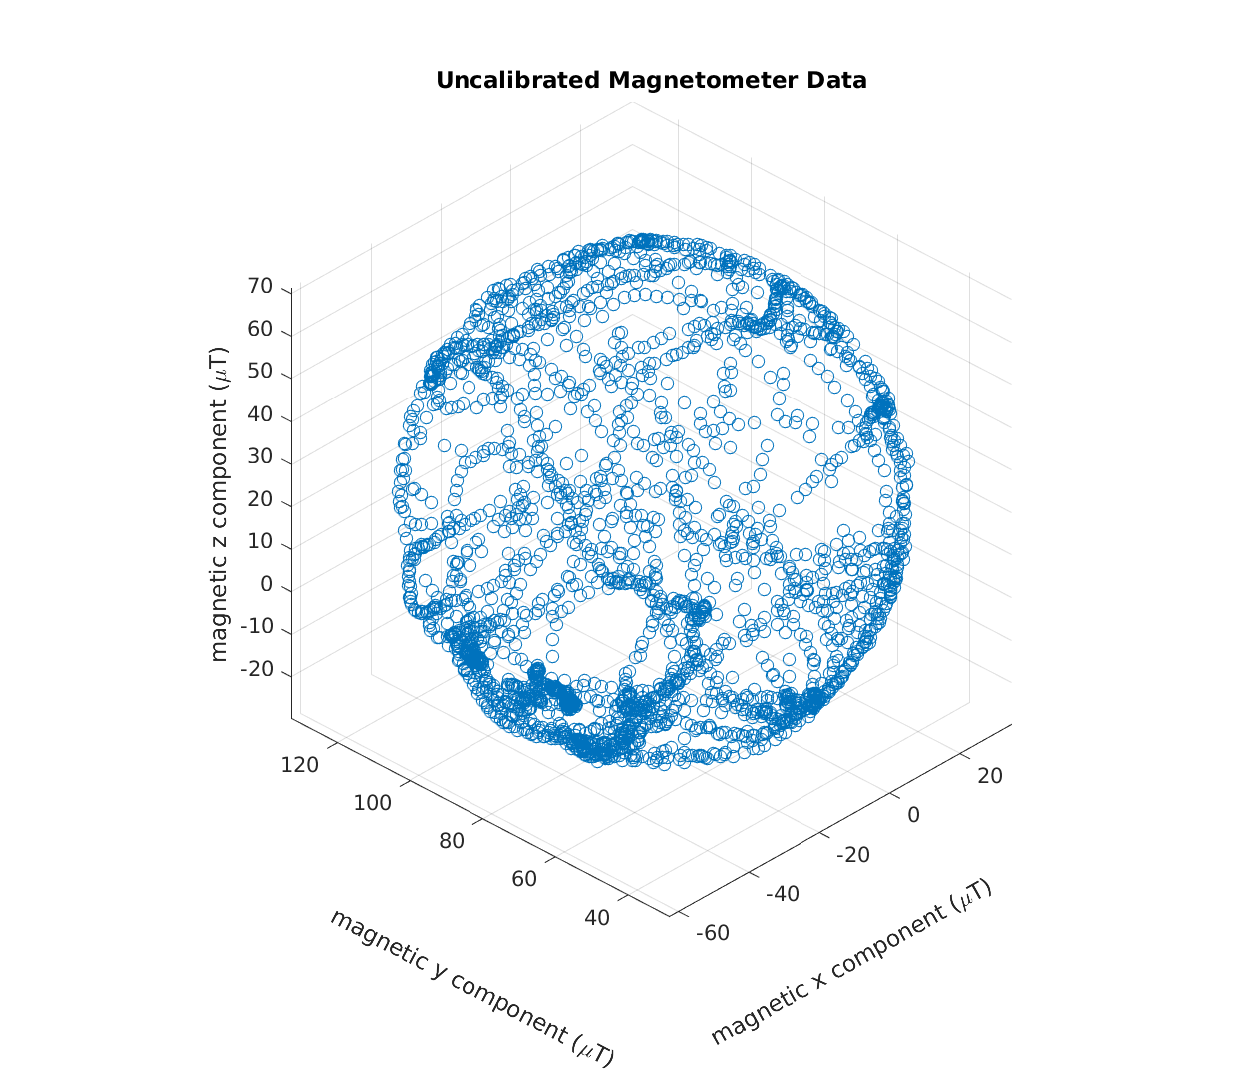
\includegraphics[trim=80 0 80 0, clip,width=1.1\linewidth]{images/20201020_1125_Uncalibrated_Magnetometer_Data}
		\caption{Uncalibrated magnetometer data}
		\label{fig:uncalibrated_magnetometer_data}
	\end{subfigure}
	\begin{subfigure}[t]{0.45\textwidth}
		\centering
		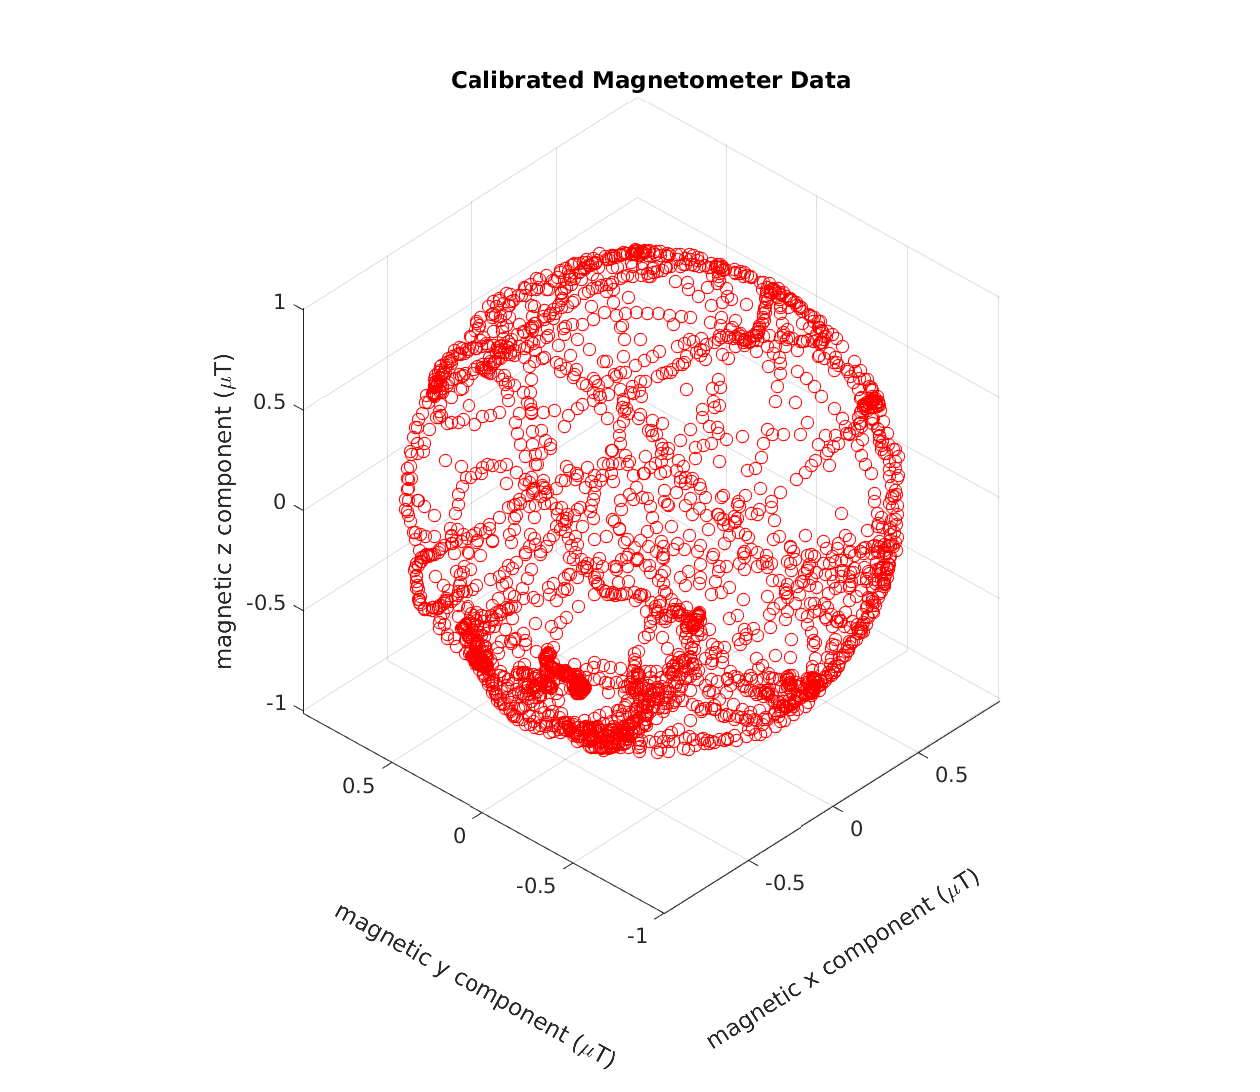
\includegraphics[trim=80 0 80 0, clip,width=1.1\linewidth]{images/20201020_1125_Calibrated_Magnetometer_Data}
		\caption{ Calibrated magnetometer data}
		\label{fig:calibrated_magnetometer_data}
	\end{subfigure}
\setlength{\belowcaptionskip}{-20pt}
	\caption{Magnetometer calibration for smart MEMS \ac{IMU} in one location. Note how the uncalibrated magnetometer data is mapped to a unit sphere with the calibrated magnetometer data.}
	\label{fig:calibration_magnetometer}
\end{figure}



\subsection{Extended Kalman Filter using Quaternions as States}
\label{sec:rw-EKF}

The Extended Kalman Filter (EKF) is a sensor fusion approach that estimates the states of non-linear models, making it appropriate for the inertial based orientation model outlined in \eqref{eq:orient_state_space}. The EKF uses the motion model to predict the orientation, while using the measurement models to calibrate it once a relevant measurement is received \cite{Kok2017}. \par 
The EKF consists of three steps, with the last two steps performed recursively.  These include similar steps as with the previously presented Particle Filter, also a sensor fusion method. The steps include initialization, time update and measurement update, explained next, with formulas originating from \cite{Kok2017}. \par 

\subsubsection{Initialization}
 Initialization requires defining an initial unit quaternion state, the variance of the process and measurement noise, and an initial state covariance representing the accuracy of the initial state. The EKF assumes that the noise affecting the state space model is additive and that both process and measurement noise are Gaussian and zero mean \cite{Kok2017}.

\subsubsection{Time Update}

A time update occurs every time a gyroscope measurement $y_\omega$ is received. It calculates a one step ahead estimate of the state vector using \eqref{eq:orient_dynamics} and its covariance matrix $P$. The calculations are as followed: 

\begin{subequations}
	\begin{align}
		\hat{q}_{k | k-1}^{\mathrm{nb}}=\hat{q}_{k-1 | k-1}^{\mathrm{nb}} \odot \exp _{\mathrm{q}}\left(\frac{k}{2} y_{\omega, k-1}\right) \\
		P_{k | k-1}=F_{k-1} P_{k-1 | k-1} F_{k-1}^{\top}+G_{k-1} \Sigma_\omega G_{k-1}^{\top}
	\end{align}
	with $ \Sigma_\omega = e_{\omega}$ as the noise covariance matrix of the gyroscope measurements, which is defined in \eqref{eq:orient_ss_noise}. Here
	\begin{align}
		F_{k-1}&=\left(\exp _{q}\left(\frac{k}{2} y_{\omega, k-1}\right)\right)^{R},\\
		G_{k-1}&=-\frac{k}{2}\left(\hat{q}_{k-1 | k-1}^{\mathrm{nb}}\right)^{L} \frac{\partial \exp _{q}\left(e_{\omega, k-1}\right)}{\partial e_{\omega, k-1}},
	\end{align}
\end{subequations}
where the $*^L$ and $*^R$ operators are defined as 
\begin{subequations}
	\begin{equation}
		q^L = \left(\begin{array}{cc}{q_{0}} & {-q_{v}^{\top}} \\ {q_{v}} & {q_{0} \mathcal{I}_{3}+\left[q_{v} \times\right]}\end{array}\right),
	\end{equation}	
	\begin{equation}
		q^R = \left(\begin{array}{cc}{q_{0}} & {q_{v}^{\top}} \\ {-q_{v}} & {q_{0} \mathcal{I}_{3}+\left[q_{v} \times\right]}\end{array}\right).
	\end{equation}
\end{subequations}

\subsubsection{Measurement Update}
The third step of the EKF is the measurement update, in which the estimate generated by the time update is compared with actual accelerometer and magnetometer measurements. Discrepancies between the two will lead to an error measurement. This error can then be used to mitigate drift in the orientation estimate. \par 
For orientation estimation using an EKF, a measurement update occurs every time an accelerometer or magnetometer reading is received. These measurements $ y_k $ are compared to what the model predicts these measurements to be, $ \hat{y}_{k | k-1}  $, using
\begin{subequations}
	\begin{equation}
		\varepsilon_{k} = y_{k}-\hat{y}_{k | k-1},
	\end{equation}
	
	where $ \varepsilon_{k} $ representing the measurement error, and where 
	
	\begin{align}
		y_{k}&=\left(\begin{array}{l}
			y_{\mathrm{a}, k} \\
			y_{\mathrm{m}, k}
		\end{array}\right),\\
		\hat{y}_{k | k-1}&=\left(\begin{array}{c}
			-\hat{R}_{k | k-1}^{\mathrm{bn}} g^{\mathrm{n}} \\
			\hat{R}_{k | k-1}^{\mathrm{bn}} m^{\mathrm{n}}
		\end{array}\right).
		\label{eq:EKF_meas_update}
	\end{align}
\end{subequations}

Here the calculations in \eqref{eq:EKF_meas_update} come from the measurement models in \cref{sec:motion_and_measurement_models}.\par 

The state correction from the resulting error is as followed:

\begin{subequations}
	\begin{align}
		\tilde{q}_{k | k}^{\mathrm{nb}} &=\hat{q}_{k | k-1}^{\mathrm{nb}}+K_{k} \varepsilon_{k}, \\
		\tilde{P}_{k | k} &=P_{k | k-1}-K_{k} S_{k} K_{k}^{\top},
	\end{align}
	with $ K_{k} $ being the Kalman gain, defined as
	\begin{align}
		K_{k} &= P_{k | k-1} H_{k}^{\top} S_{k}^{-1},\\
		S_{k} &= H_{k} P_{k | k-1} H_{k}^{\top}+R.		
	\end{align}
	\label{eq:quat_meas_update}	
	
	where
	
	\begin{align}
		H_{k}&=\left.\frac{\partial}{\partial q_{k}^{\mathrm{nb}}}\left(\begin{array}{c}{R_{k}^{\mathrm{bn}} g^{\mathrm{n}}} \\ {R_{k}^{\mathrm{bn}} m^{\mathrm{n}}}\end{array}\right)\right|_{q_{k}^{\mathrm{nb}}=\hat{q}_{k | k-1}^{\mathrm{nb}}}, \\
		&= \left(
		\begin{array}{l}
			-\left.\frac{\partial R_{k | k-1}^{\mathrm{bn}}}{\partial q_{k | k-1}^{\mathrm{nb}}}\right|_{{q_{k | k-1}^{\mathrm{nb}}}=\hat{q}_{k | k-1}^{\mathrm{nb}}} \quad g^{\mathrm{n}}\\
			\left.\frac{\partial R_{k | k-1}^{\mathrm{bn}}}{\partial q_{k | k-1}^{\mathrm{nb}}}\right|_{{q_{k | k-1}^{\mathrm{nb}}}=\hat{q}_{k | k-1}^{\mathrm{nb}}} \quad m^{\mathrm{n}}
		\end{array}
		\right).
	\end{align}

and 

\begin{equation}\label{key}
	R = \left[\begin{array}{cc}
		\Sigma_a & 0 \\
		0 & \Sigma_m
	\end{array} \right]
\end{equation}

	with $ \Sigma_a = e_{a}$ and $ \Sigma_m = e_{m}$ as the noise covariance matrix of the accelerometer and magnetometer measurements, respectively.

\end{subequations}

Once a measurement update occurs the resulting quaternion is not necessarily a unit quaternion, which is a requirement for orientation parametrization. To facilitate this, a renormalization of the quaternion is required, using

\begin{equation}
	\hat{q}_{k | k}^{\mathrm{nb}}=\frac{\tilde{q}_{k-1}^{\mathrm{nb}}}{\left\|\tilde{q}_{k | k}^{\mathrm{nb}}\right\|_{2}}.
\end{equation}
